\begin{frame}
\frametitle{Simpler concept: the ABCD method}
\begin{center}
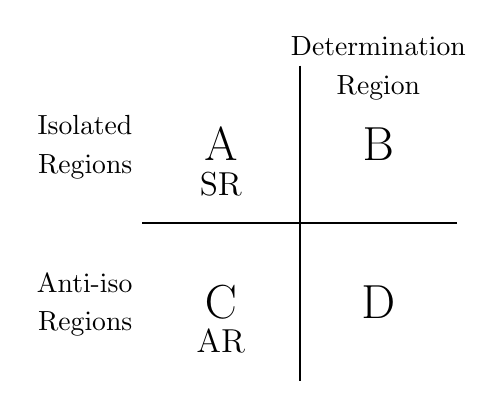
\begin{tikzpicture}
\def\hdAB{1}
\draw (-\hdAB,\hdAB) coordinate (A);
\draw (\hdAB,\hdAB) coordinate (B);
\draw (-\hdAB,-\hdAB) coordinate (C);
\draw (\hdAB,-\hdAB) coordinate (D);

\draw (-\hdAB,\hdAB/2) coordinate (SR);
\draw (-\hdAB,-3*\hdAB/2) coordinate (AR);

\draw [thick] (0,2*\hdAB)--(0,-2*\hdAB);
\draw [thick] (2*\hdAB,0)--(-2*\hdAB,0);

\foreach \coord in {A,B,C,D}{\draw(\coord)node{\LARGE\coord};}
\foreach \coord in {SR,AR}{\draw(\coord)node{\large\coord};}

\draw (\hdAB,2*\hdAB) node [above] {Determination} node [below] {Region};

\draw (-2*\hdAB,\hdAB) node [above left] {Isolated} node [below left] {Regions};
\draw (-2*\hdAB,-\hdAB) node [above left] {Anti-iso} node [below left] {Regions};
\end{tikzpicture}
\end{center}
\pause
\begin{minipage}{.5\textwidth}
\begin{block}{Hypothesis}
\begin{itemize}
\item $\displaystyle\frac{N_\text{A}}{N_\text{C}}=\frac{N_\text{B}}{N_\text{D}}=\mathrm{FF}$
\item Shapes are isolation-independents.
\end{itemize}
\end{block}
\end{minipage}
\begin{minipage}[c]{.49\textwidth}\Large
\pause
\begin{equation*}
\Rightarrow
\boxed{\text{histo}_\text{SR} = \mathrm{FF} \times \text{histo}_\text{AR}}
\end{equation*}
\end{minipage}
\end{frame}
